\documentclass[a4paper,12pt]{article}
\usepackage[utf8]{inputenc}
\usepackage[cm,empty]{fullpage}
\usepackage[T2A]{fontenc}
\usepackage[english, russian]{babel}
\usepackage{amssymb,amsmath,amsxtra,amsthm}
\usepackage{proof}
\usepackage[pdftex]{graphicx}
\usepackage{wrapfig}
\usepackage{braket}
\usepackage{xcolor}
\usepackage{enumitem}

\usepackage[left=2cm,right=2cm,
    top=1cm,bottom=1cm,bindingoffset=0cm]{geometry}

\renewcommand{\leq}{\leqslant}
\renewcommand{\geq}{\geqslant}


\newcommand{\iiff}{\Longleftrightarrow}
\renewcommand{\iff}{\Leftrightarrow}
\newcommand{\nothing}{\varnothing}

\newtheorem*{rem}{Замечание}

\newcommand{\NN}{\mathbb{N}}
\newcommand{\ZZ}{\mathbb{Z}}
\newcommand{\Q}{\mathbb{Q}}
\newcommand{\A}{\mathbb{A}}
\newcommand{\R}{\mathbb{R}}
\renewcommand{\C}{\mathbb{C}}

\renewcommand{\phi}{\varphi}
\newcommand{\eps}{\varepsilon}

\makeatletter
\newcommand*{\rom}[1]{\expandafter\@slowromancap\romannumeral #1@}
\makeatother

\newcounter{z}


\newcommand{\zs}{\refstepcounter{z}\vskip 10pt\par\noindent
\fbox{\textbf{12.\arabic{z}}} }

\newcommand{\z}{\refstepcounter{z}\vskip 20pt\noindent
\fbox{\textbf{\arabic{z}}} }

\renewcommand{\date}{{\bf 12 июня 2021}} 

\newcommand{\dif}
{
------------------------------------------------------------------------------------------------------------------------------------------------------
}

\newcommand{\HSEhat}{
\vspace*{-0pt}
\noindent
\setcounter{z}{0}


{\bf \phantom{\date}  \large \hfill Теория вероятностей: \hfill \normalsize \date}

\vspace{5 pt}
{\bf \large \hfill  лекция 5\hfill }

\vspace{15 pt}
\centerline{ \large  Домашнее задание.}
\centerline{ \large  Кирилл Сетдеков}



\vspace*{10pt}
\setcounter{z}{0}

}

\begin{document}
\HSEhat


\begin{enumerate}

\subsection*{Задачи:}

\item Идеальная игральная кость бросается 100 раз. Найдите вероятность того, что сумма всех выпавших номеров окажется в пределах от 330 до 380. 

\textbf{Решение:}\\
Пусть $X \sim $ дискретная случайная величина, отражающая значения с 1 кубика. Тогда: $EX = 3.5; DX = \frac{35}{12}$. Если $Y=\sum_{i=1}^{100} X_i$ - случайная величина суммы на 100 кубиках, то $EY =350; DY=291\frac{2}{3}; \sigma (Y) = \sqrt{DY}=5\sqrt{\frac{35}{3}}$.

По ЦПТ, предположим, что число кубиков достаточно большое, поэтому сумма уже нормально распределена. Запишем нужную вероятность и найдем ответ:
$$P(330<Y<380)=\Phi(\frac{380-EY}{\sigma (Y)})-\Phi(\frac{330-EY}{\sigma (Y)})=\Phi(\frac{380-350}{5\sqrt{\frac{35}{3}}})-\Phi(\frac{330-350}{5\sqrt{\frac{35}{3}}})=$$
$$=\Phi(1.757)-\Phi(-1.171)=0.961-0.121=0.840$$

\textbf{Ответ: вероятность получить сумму в интервале от 330 до 380 = 0.84} 

\item Допустим, что расстояния между автомобилями, движущимися в одном направлении по некоторому шоссе, экспоненциально распределены со средним значением 100 метров. Какова вероятность того, что на отрезке шоссе длиной в 5 километров находятся от 50 до 60 автомобилей? 

\textbf{Решение:}\\
Пусть X - случайная величина, отвечающая за расстояние от автомобиля до следующего, которая распределена экспоненциально с $\lambda=1/100$. Тогда $EX =100; DX = 10000$. Нас интересует расстояние в 5 км. В среднем это будет 50 машин. Введем $Y=50X$, тогда $EY=5000; DY=500000; \sigma (Y) = 500\sqrt{2}$.
50 Машин на 5 км, будут соответствовать Y=5000, а 60 машин на 5 км будут соответствовать $Y=\frac{5000 \cdot 50}{60} = 4166 \frac{2}{3}$.

Решим через ЦПТ:\\
Запишем вопрос из условия:
$$P(4166 \frac{2}{3} < Y < 5000)=\Phi(\frac{5000-EY}{\sigma (Y)})-\Phi(\frac{4166 \frac{2}{3}-EY}{\sigma (Y)})=$$
$$=\Phi(0)-\Phi(-1.179)=0.5-0.119=0.381$$

Через $\Gamma$\\
Мы знаем, что для распределения, состоящего из суммы экспоненциальных распределений есть функция $\Gamma$ распределения. В этом примере, параметры $\alpha = 50; \lambda=1/100$:
$$P(4166 \frac{2}{3} < Y < 5000)=CDF_{\Gamma(\alpha = 50; \lambda=1/100)}(5000)-CDF_{\Gamma(\alpha = 50; \lambda=1/100)}(4166 \frac{2}{3})=$$
$$=0.518-0.114=0.404$$

\textbf{Ответ: вероятность, оцененная по ЦПТ = 0.381. Вероятность, оцененная через Гамма распределение = 0.404} 

\item В продукции цеха детали отличного качества составляют 50\%. Детали укладываются в коробки по 200 шт. в каждой. Какова вероятность того, что число деталей отличного качества в коробке отличается от 100 не более, чем на 15

\textbf{Решение:}\\
Пусть $X\sim$ биномиальное распределение с n=100 и p=0.5. Которое соответствует числу отличных деталей в коробке. $EX=np=100; DX = npq = 50; \sigma(X) = 5\sqrt{2}$ .\\
Используем ЦПТ и перейдем к нормальному распределению, чтобы решить задачу, так как n велико:
$$P(85<X<115)=\Phi(\frac{115-EX}{\sigma (X)})-\Phi(\frac{85-EX}{\sigma (X)})=\Phi(\frac{115-100}{5\sqrt{2}})-\Phi(\frac{85-100}{5\sqrt{2}})=$$
$$=\Phi(2.121)-\Phi(-2.121)=0.983-0.017=0.966$$

\textbf{Ответ: вероятность получить число отличных деталей, отличное от 100 менее, чем на 15, оцененная по ЦПТ = 0.966.} 

\item Два кинотеатра вмещают 1 000 зрителей. Допустим, что каждый зритель выбирает один из кинотеатров случайно и независимо от других зрителей. Сколько мест необходимо иметь в каждом кинотеатре, чтобы вероятность того, что какому-то зрителю не удастся попасть на сеанс из-за отсутствия мест, была не более 1\% ?

\textbf{Решение:}\\
1000 человек расходятся по 2 кинотеатрам. Пусть X - число мест в первом кинотеатре, Y - число мест в 2-м кинотеатре. А $V\sim$ биномиальная случайная величина, показывающая сколько человек пошло в кинотеатр 1.
$EV = np =500; DV = npq = 250; \sigma(V) = 5 \sqrt{10}$

Используем ЦПТ и записываем задачу ограничения:
$$P(X<V) + P(Y<V) < 0.01$$
так как одинаковая вероятность пойти в первый или второй кинотеатр, можно предположить, что $P(X<V)=P(Y<V)$ и $X=Y$, что сведет нашу задачу к:
$$P(X<V)  < 0.005 \Rightarrow$$
$$1- P(V<X)  < 0.005 \Rightarrow$$
$$1- \Phi(\frac{X-EV}{\sigma (V)})  < 0.005 \Rightarrow$$
$$\frac{X-EV}{\sigma (V)}  < \Phi^{-1}(0.995)  \Rightarrow$$
$$X > 500+ \Phi^{-1}(0.995) \cdot \sigma (V) = 500+2.58 \cdot 15.81 = 540.7$$

\textbf{Ответ: если в каждом из кинотеатров будет 541 место или больше, вероятность каждому из зрителей не попасть на сеанс будет менее 1\%} 




\item Срок службы электрической лампы имеет показательное распределение с математическим ожиданием 1000 часов. Найти вероятность того, что средний срок службы для 100 ламп составит не менее 900 часов. 

\textbf{Решение:}\\
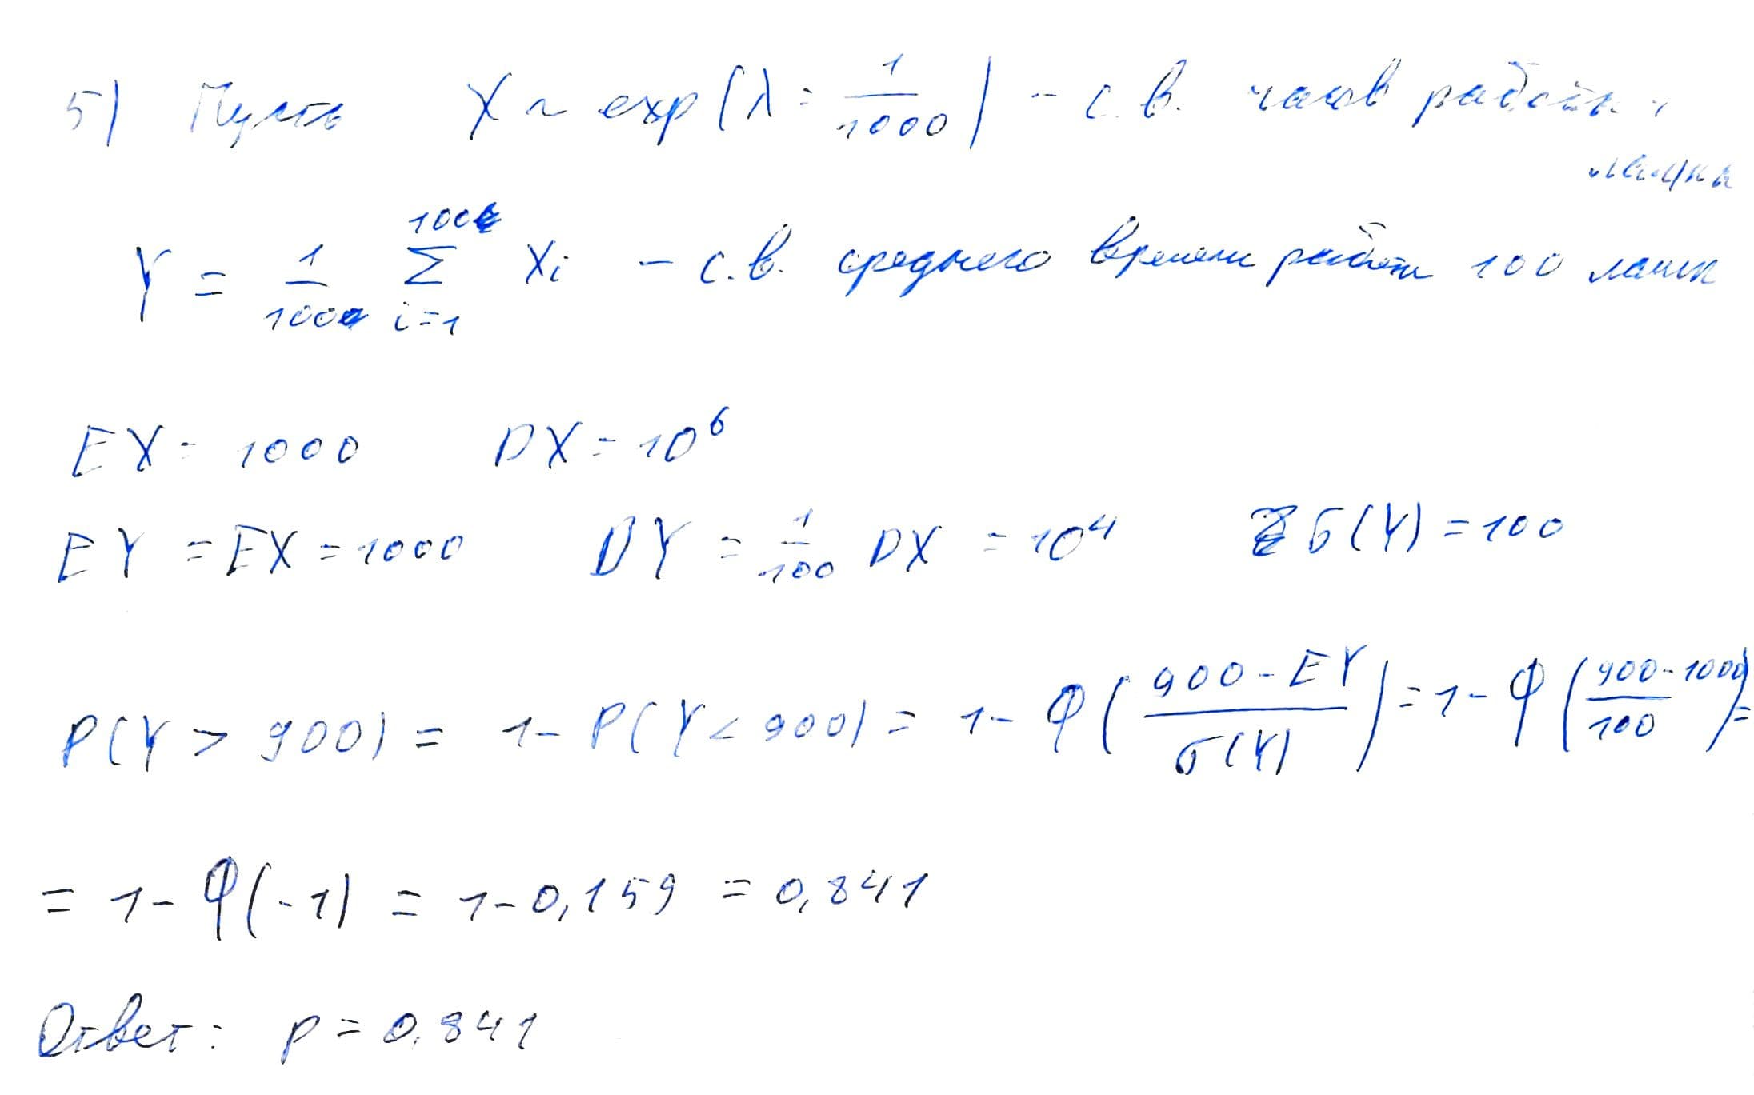
\includegraphics[width=\textwidth]{img/hw5t5.pdf}
\textbf{Ответ: $p \approx 0.841 $} 


\item В городе за год рождается 20 000 детей и считается, что вероятность рождения мальчика p = 0.51. В этом случае существует такое число d, что среди рожденных за год детей разница числа мальчиков и числа девочек будет не больше d с вероятностью 0.99. Найдите это d.

\textbf{Решение:}\\

Пусть X - число мальчиков, W - число девочек в этом городе, $C=X-W$ - разница числа мальчиков и девочек. 

Тогда из свойств биномиального распределения:
$EX=np = 10200; EW = nq = 9800; DX=DW = npq=4998$.

$EC = 400$, $DC = DX + DW -2 Cov(X,W)$\\
С ковариацией мы можем сказать следующее: $Corr(X,W)=-1$, так как эти числа линейно зависимые, следовательно $Cov(X,W) = Corr(X,W)\sigma(X)\sigma(Y)=-DX$ так как дисперсии равны, то и стандартные отклонения равны. Следовательно $DC=2DX- -2DX = 4DX$. $\sigma(C) = 2\sqrt{4998}$.

Согласно ЦПТ, решим задание.
$$P(C<d) = 0.99 \Rightarrow$$
$$\Phi(\frac{d-400}{\sigma(C)})=0.99 \Rightarrow$$
$$\frac{d-400}{\sigma(C)}=\Phi^{-1}(0.99) \Rightarrow$$

$\Phi^{-1}$ - функция обратного нормального стандартного распределения. Посчитаем ответ:
$$d = 400+\sigma(C) \cdot \Phi^{-1}(0.99) = 400 + 141.39 \cdot 2.33 \approx 728.9 $$

\textbf{Ответ: $d \approx 728.9 $} 

\end{enumerate}
\end{document}